\chapter{前提知識}

\section{生体リズム研究}

\cite{koriAcceleratingRecoveryJet2017}

\cite{yamaguchiMiceGeneticallyDeficient2013a}

\section{力学系}
一般的な話.
\cite{strogatz2018nonlinear}とかを参考に一般論.


\subsection{Van Der Polモデル}

\begin{align}
    \frac{d^2 x}{d t^2}-\mu\left(1-x^2\right) \frac{d x}{d t}+x=0
\end{align}



\subsection{Rösslerモデル}
\clearpage
\section{Reservoir Computerの概要}

Reservoir ComputerはEcho State Network (ESN)の一つのモデルである.ESNはRecurrent Neural Network (RNN)の枠組みの一つで,学習の対象を出力層のみに限定することによって,従来のRNNと比較して学習コストを大幅に節約する.
ここでは,\cite{bolltExplainingSurprisingSuccess2021}に基づいて,Reservoir Computerの構造と原理について概説する.また,Reservoir Computerの理論的な背景についても,先行研究を交えながら触れる.

\textbf{構造.}
Reservoir Computerは,入力層(Input layer),レザバー層(Reservoir layer),出力層(Output/ Readout Layer)の三つの層から成る.


\begin{figure}[h]
    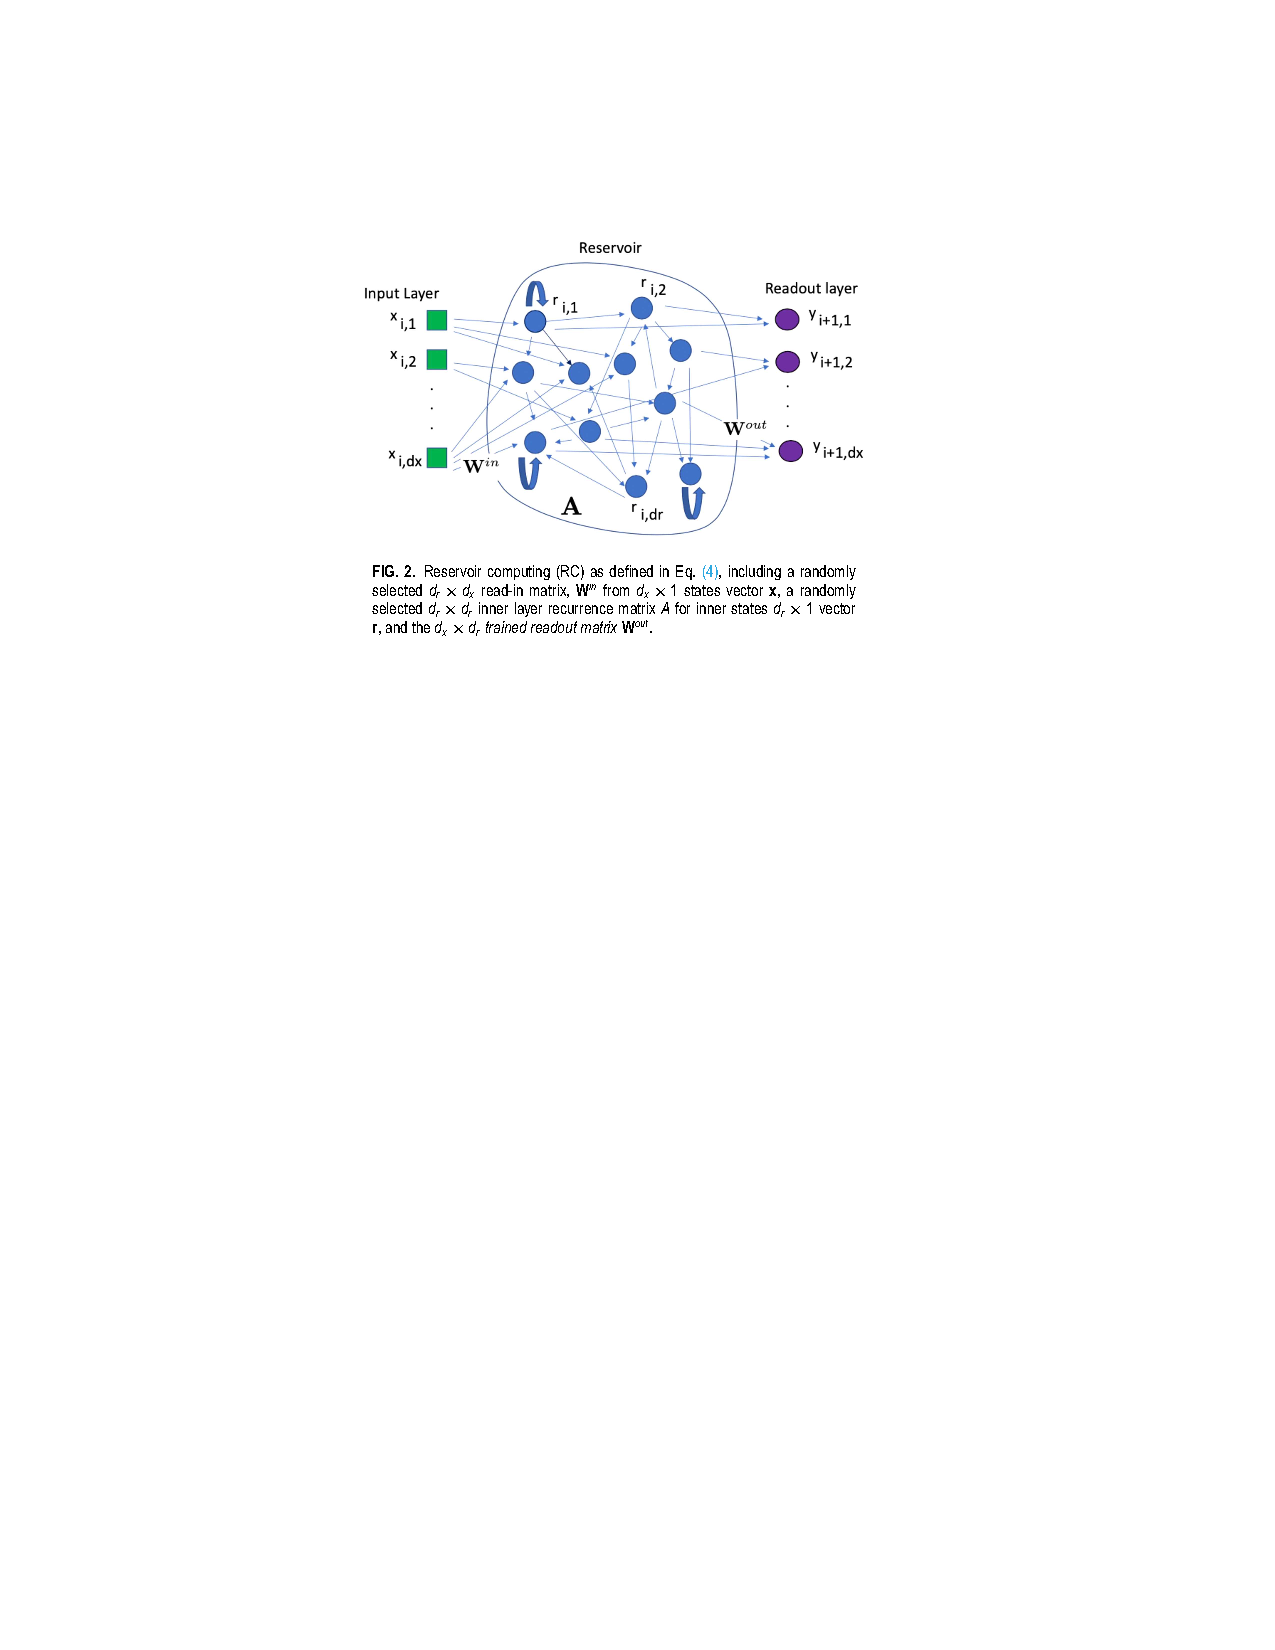
\includegraphics[width=\textwidth]{images/bollt.reservoir.pdf}
    \caption{}
\end{figure}  


\textbf{原理.}


\begin{comment}
    \begin{figure}[h]
    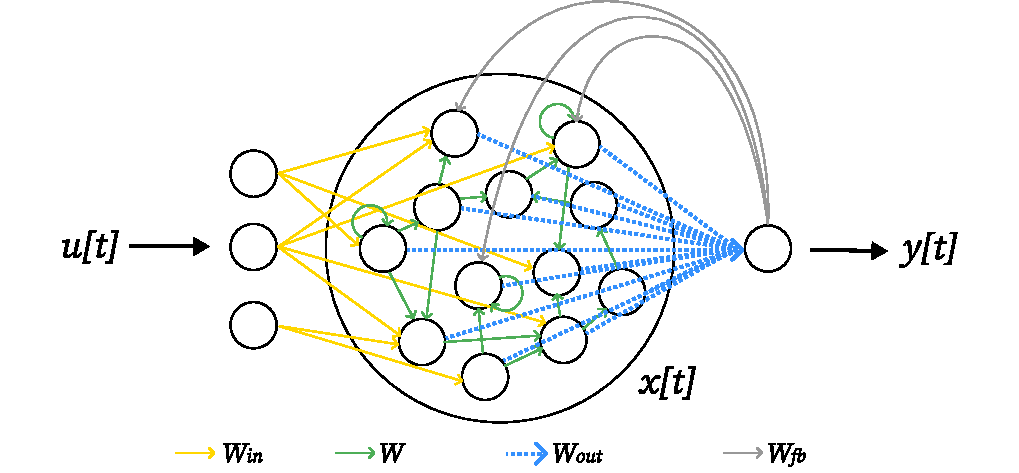
\includegraphics[width=\textwidth]{images/esn.pdf}
\end{figure}  
\begin{figure}[h]
    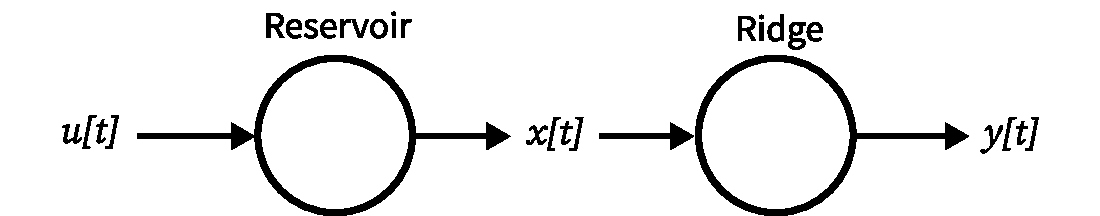
\includegraphics[width=\textwidth]{images/esn_nodes.pdf}
    \caption{}
\end{figure}  
\end{comment}


\textbf{理論的な背景.}
\cite{grigoryevaChaosCompactManifolds2021}
\cite{grigoryevaLearningStrangeAttractors2023}
\cite{berryLearningTheoryDynamical2023a}

Stochastic Inputsに対するuniversal approximationの話.
\cite{grigoryevaUniversalDiscretetimeReservoir2018}




\clearpage
\section{応用面での先行研究}


比較検討論文.二つくらいあってもいいかな.
\cite{zhangSurveyReservoirComputing2023}:Online learning/ force algorithm等に触れている.



\subsection{Y. Laiの研究内容}
本研究の直接的な先行研究として\cite{kongDigitalTwinsNonlinear2022}があるので,ここでその内容について紹介する.

\begin{figure}[h]
    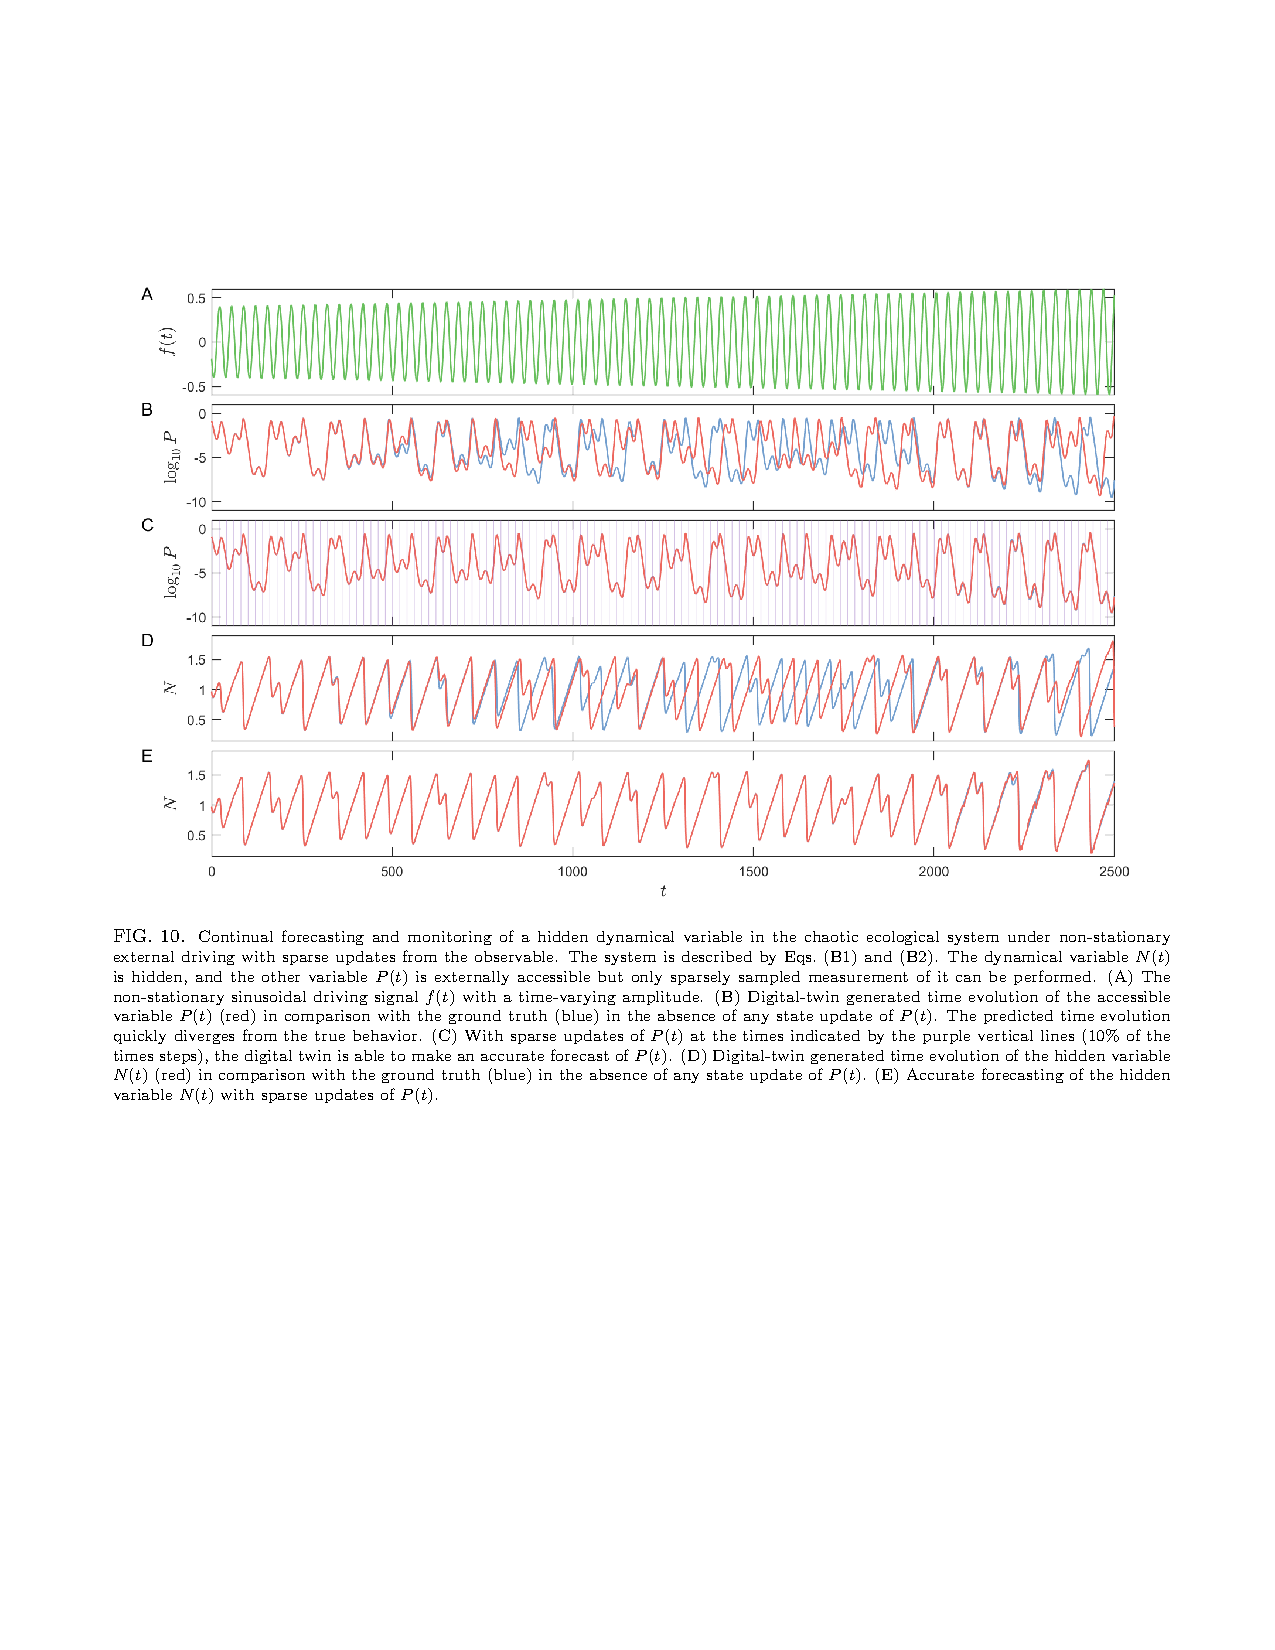
\includegraphics[width=\textwidth]{images/lai_result.pdf}
    \caption{}
\end{figure}  


\clearpage